% Standalone source for figures/price_sweep.pdf (P(GO) by bus fare; points only, no CIs). Build: tectonic price_sweep.tex
% Data: figures/price_sweep_data.csv (generated from mini_study/runs). x = log(1 + fare).
\documentclass[border=2pt]{standalone}
\usepackage{times}
\usepackage{pgfplots}
\pgfplotsset{compat=1.18}
\definecolor{c0}{HTML}{2a78d6}
\definecolor{c1}{HTML}{eb6834}
\definecolor{c2}{HTML}{1baf7a}
\definecolor{c3}{HTML}{eda100}
\definecolor{c4}{HTML}{e87ba4}
\definecolor{c5}{HTML}{008300}
\definecolor{c6}{HTML}{6250d6}
\begin{document}
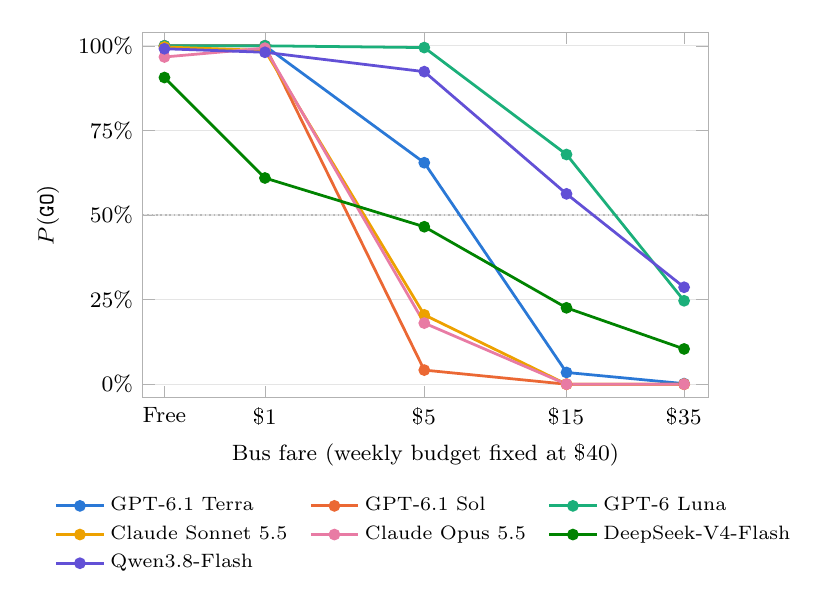
\begin{tikzpicture}
\begin{axis}[
  width=3.45in, height=2.45in,
  xmin=-0.15, xmax=3.75, ymin=-4, ymax=104,
  xtick={0, 0.6931, 1.7918, 2.7726, 3.5835},
  xticklabels={Free, \$1, \$5, \$15, \$35},
  ytick={0,25,50,75,100}, yticklabel={\pgfmathprintnumber{\tick}\%},
  xlabel={Bus fare (weekly budget fixed at \$40)}, ylabel={$P(\texttt{GO})$},
  label style={font=\footnotesize}, tick label style={font=\footnotesize},
  axis line style={gray!60}, tick style={gray!60},
  ymajorgrids, grid style={gray!20, line width=0.4pt},
  legend style={font=\scriptsize, draw=none, fill=none, at={(0.5,-0.24)}, anchor=north, legend columns=3,
                /tikz/every even column/.append style={column sep=6pt}},
  legend cell align=left, clip=false,
]
\draw[gray!55, densely dotted, line width=0.6pt] (axis cs:-0.15,50) -- (axis cs:3.75,50);
\addplot[c0, solid, line width=1pt, mark=*, mark size=1.6pt, mark options={solid, fill=c0}] coordinates {(0.0000,100.00) (0.6930,100.00) (1.7920,65.45) (2.7730,3.47) (3.5840,0.17)};
\addlegendentry{GPT-6.1 Terra}
\addplot[c1, solid, line width=1pt, mark=*, mark size=1.6pt, mark options={solid, fill=c1}] coordinates {(0.0000,100.00) (0.6930,100.00) (1.7920,4.17) (2.7730,0.00) (3.5840,0.00)};
\addlegendentry{GPT-6.1 Sol}
\addplot[c2, solid, line width=1pt, mark=*, mark size=1.6pt, mark options={solid, fill=c2}] coordinates {(0.0000,100.00) (0.6930,100.00) (1.7920,99.48) (2.7730,67.88) (3.5840,24.65)};
\addlegendentry{GPT-6 Luna}
\addplot[c3, solid, line width=1pt, mark=*, mark size=1.6pt, mark options={solid, fill=c3}] coordinates {(0.0000,99.65) (0.6930,98.61) (1.7920,20.49) (2.7730,0.00) (3.5840,0.00)};
\addlegendentry{Claude Sonnet 5.5}
\addplot[c4, solid, line width=1pt, mark=*, mark size=1.6pt, mark options={solid, fill=c4}] coordinates {(0.0000,96.70) (0.6930,99.31) (1.7920,18.06) (2.7730,0.00) (3.5840,0.00)};
\addlegendentry{Claude Opus 5.5}
\addplot[c5, solid, line width=1pt, mark=*, mark size=1.6pt, mark options={solid, fill=c5}] coordinates {(0.0000,90.63) (0.6930,60.94) (1.7920,46.53) (2.7730,22.57) (3.5840,10.42)};
\addlegendentry{DeepSeek-V4-Flash}
\addplot[c6, solid, line width=1pt, mark=*, mark size=1.6pt, mark options={solid, fill=c6}] coordinates {(0.0000,99.13) (0.6930,98.09) (1.7920,92.36) (2.7730,56.25) (3.5840,28.65)};
\addlegendentry{Qwen3.8-Flash}
\end{axis}
\end{tikzpicture}
\end{document}
